\documentclass[8pt]{beamer}

\usepackage[utf8]{inputenc}
\usepackage{eurosym}
\RequirePackage[francais]{babel}
%\usepackage{url}
%\usepackage{etex}
%\usepackage{enumitem}
%\usepackage{multicol}
\usepackage{xcolor}
%\usepackage{bbm}
%\usepackage{amsmath,amsthm,amssymb}
%\usepackage[official]{eurosym}
\usepackage{pifont}
%\usepackage{exercise}
%\usepackage{graphics}
%\usepackage{array,multirow,makecell}
\usepackage{verbatim}
%\usepackage[dvipsnames]{pstricks}
\usepackage{pstricks-add,pst-plot,pst-text,pst-tree,pst-eps,pst-fill,pst-node,pst-math,pst-blur,pst-func}
%\usepackage{pgf,tikz}
%\usepackage{tipfr}
%\usepackage{thmbox}
%\usepackage{calc}
%\usepackage{ifthen}
%\usepackage{pdfpages}
%\usepackage{colortbl}
%\usepackage{sagetex}
%\usetikzlibrary{arrows,patterns}
%\input tabvar
%\usepackage{tkz-tab}
%\usepackage{listings}
%\usepackage[np]{numprint}
%\usepackage{fancybox,fancyhdr}
%\usepackage{thmtools}
%\usepackage{bclogo}
%\usepackage{lastpage}

\usepackage{tabularx}
\usepackage{array,multirow,makecell}
\usetheme{Madrid}
%\usetheme{Bergen}
\usecolortheme{beaver}
 
%Information to be included in the title page:
\title{WEB}
\subtitle{HTML - CSS - JAVASCRIPT}
\author{Yannick CHISTEL}
\institute{Lycée Dumont d'Urville - CAEN}
\date{Janvier 2020}
 
%----------------------------------------------------------------------------------------------- 
% 							Commandes Tableaux
%-----------------------------------------------------------------------------------------------
\setcellgapes{1pt}
\makegapedcells
\newcolumntype{R}[1]{>{\raggedleft\arraybackslash }b{#1}}
\newcolumntype{L}[1]{>{\raggedright\arraybackslash }b{#1}}
\newcolumntype{C}[1]{>{\centering\arraybackslash }b{#1}}

\definecolor{vert}{rgb}{0,0,1}


\newcounter{num}
\setcounter{num}{0}
 
\begin{document}
 
\frame{\titlepage}

\begin{frame}
\frametitle{Fonctionnement du WEB}


\begin{block}{Introduction}
Le mot WEB est une abréviation de l'expression World Wide WEB qui signifie \og toile d'araignée de taille mondiale \fg.

Le principe du WEB consiste à relier des documents entre eux via des liens hytpertextes. Un lien hypertexte est un mot, une phrase ou une image qui permet d'accéder au document vers lequel il renvoie. 

Pour afficher et lire un document du WEB, on utilise un logiciel appelé \textbf{navigateur}. Il en existe de nombreux comme FIREFOX, CHROME, EDGE, OPERA,...
\end{block}

\begin{block}{Langages du WEB}
Différents langages sont utilisés pour structurer et afficher les documents du WEB :
\begin{itemize}
\item Le langage HTML qui est composé du contenu et de la structure du document à afficher par le navigateur ; 
\item Le langage CSS qui assure la mise en page et l'apparence graphique du document ;
\item Le langage JAVASCRIPT qui permet d'ajouter de l'interactivité au document.
\end{itemize}
\end{block}

\end{frame}


\begin{frame}
\frametitle{Langage HTML}

\begin{block}{Définition}
HTML est l'acronyme de Hyper Text Markup Language signifiant Langage de Balisage Hyper Texte.

Le Langage HTML est un fichier texte qui est composé du contenu à afficher et de la structure du document selon laquelle le contenu est organisé : titre, paragraphe, emphase, liste, lien, image, etc.

Il existe une version stricte du HTML notée XHTML imposant une syntaxe plus rigoureuse que nous utiliserons.
\end{block}

\begin{block}{Balisage}
La structure du document est décrite par des balises, qui sont des mots délimités par les caractères $<$ et $>$ appelés \textit{chevrons}. On a 2 types de balises:

\begin{itemize}
\item Les balises \textbf{ouvrantes} et \textbf{fermantes }: $<balise>$ contenu $</balise>$

\textbf{Exemple}: $<\text{p}>$le contenu d'un paragraphe $</ \text{p}>$

\item Les balises \textbf{vides} : $<balise />$

\textbf{Exemple}: Pour introduire un retour à la ligne $<\text{br} />$
\end{itemize}

Les balises peuvent contenir des \textbf{attributs} qui sont des propriétés supplémentaires à appliquer au contenu à afficher.
\end{block}


\end{frame}


\begin{frame}
\frametitle{Langage HTML}

\begin{block}{Structure d'un document HTML}
Les documents HTML ont la même structure (squelette) générale.
\begin{enumerate}
\item Déclaration de type nécessaire au navigateur pour savoir que c'est un document HTML.
\item Structure du document HTML à afficher elle même décomposée en 2 parties :
\begin{itemize}
\item L'EN-TÊTE (HEAD) qui contient des informations sur le document HTML comme le titre, l'encodage de caractères, des liens vers des ressources à utiliser pour l'affichage, des scripts pour l'interactivité, etc. Ces informations ne sont pas directement visibles dans le contenu affiché.
\item LE CORPS (BODY) qui contient le contenu et la structure du document à afficher.
\end{itemize}
\end{enumerate}

\end{block}

\begin{exampleblock}{Exemple}
\begin{center}
\includegraphics[scale=0.35]{img/exemple1-code.eps}
\end{center}
\end{exampleblock}

\end{frame}




\begin{frame}
\frametitle{Langage HTML}

\begin{block}{En-tête du document}
L'en-tête contient des informations sur le document HTML comme :
\begin{itemize}
\item Le titre du document inséré entre les balises $<\text{title}>$ et $</\text{title}>$. Ce titre est affiché dans l'onglet du navigateur ou la barre d'état de la fenêtre de navigation.
\item L'encodage de caractères (ou autres informations sur le document) à utiliser inséré dans une balise vide $<\text{meta} />$ et avec l'attribut \textbf{charset} ce qui donne : $<\text{meta charset="utf-8"}/>$
\item Des liens vers des ressources externes peuvent être ajoutés avec la balise  $<\text{link}>$ et des attributs (notamment les feuilles de style CSS).
\item Des scripts JAVASCRIPT avec les balises $<\text{script}>$ et $</\text{script}>$
\end{itemize}

\end{block}

\begin{exampleblock}{Exemple}
En-tête d'un document HTML :
\begin{center}
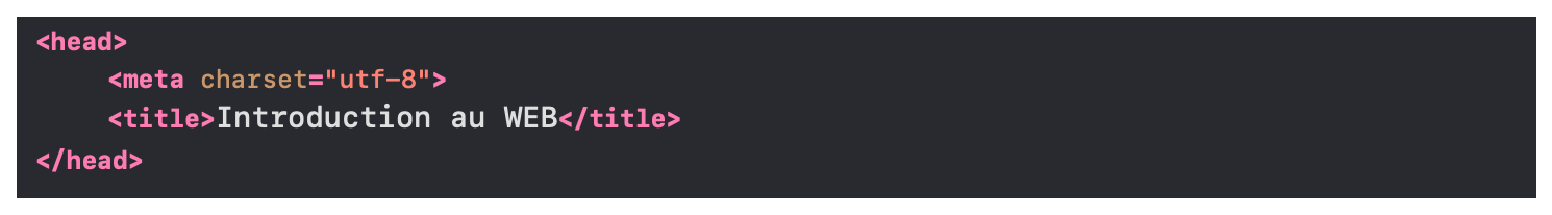
\includegraphics[scale=0.38]{img/exemple2-code.eps}
\end{center}
\end{exampleblock}

\end{frame}


\begin{frame}
\frametitle{Langage HTML}

\begin{block}{Corps du document}
Le corps (body) contient le contenu et la structure du document. On peut distinguer différents types de balises :
\begin{enumerate}
\item Les balises de structure comme le titre, le paragraphe, une liste, un tableau.
\item Les balises de texte comme le gras, l'italique, l'exposant, l'indice, le lien hypertexte, l'image.
\item Les balises de bloc pour regrouper des éléments ou organiser différents contenus dans une même page comme le contenu principal, un menu de navigation, une barre latérale de ressources, un entête de page ou un pied de page.
\end{enumerate}
\end{block}

\begin{alertblock}{Remarque}
L'association $<balise>$ contenu $</balise>$ constitue un \textbf{élément HTML}.
\begin{enumerate}
\item Un élément peut être simple avec 2 balises et un contenu.
\item Un élément peut imbriquer plusieurs éléments HTML.
\end{enumerate}
La notion d'élément HTML est importante pour le CSS et le JAVASCRIPT.
\end{alertblock}
\end{frame}

\begin{frame}
\frametitle{Langage HTML}

\begin{block}{Balises de structure}
\begin{itemize}
\item Il existe 6 niveaux de titre balisés par ordre décroissant par \textbf{h1}, \textbf{h2}, \textbf{h3}, \textbf{h4}, \textbf{h5} et \textbf{h6}
\item Le paragraphe est balisé par \textbf{p}
\item Une liste non ordonnée est balisée par \textbf{ul} et chaque item de la liste est balisé par \textbf{li}
\item Une liste ordonnée (numérotée) est balisée par \textbf{ol} et chaque item de la liste est balisé par \textbf{li}
\item Un tableau est balisé par \textbf{table}, chaque ligne est balisée par \textbf{tr} et chaque colonne est balisée par \textbf{td}
\end{itemize}


\end{block}


\begin{alertblock}{Remarque}
\begin{enumerate}
\item Les balises peuvent contenir des attributs notamment liés aux feuilles de style CSS.
\item Toutes ces balises sont ouvrantes et fermantes et entourent les contenus. Ce sont des éléments HTML.
\end{enumerate}

\end{alertblock}

\end{frame}


\begin{frame}
\frametitle{Langage HTML}

\begin{exampleblock}{Exemple:}
Voici le corps d'un document HTML contenant un titre, 2 paragraphes et une liste numérotée:
\begin{center}
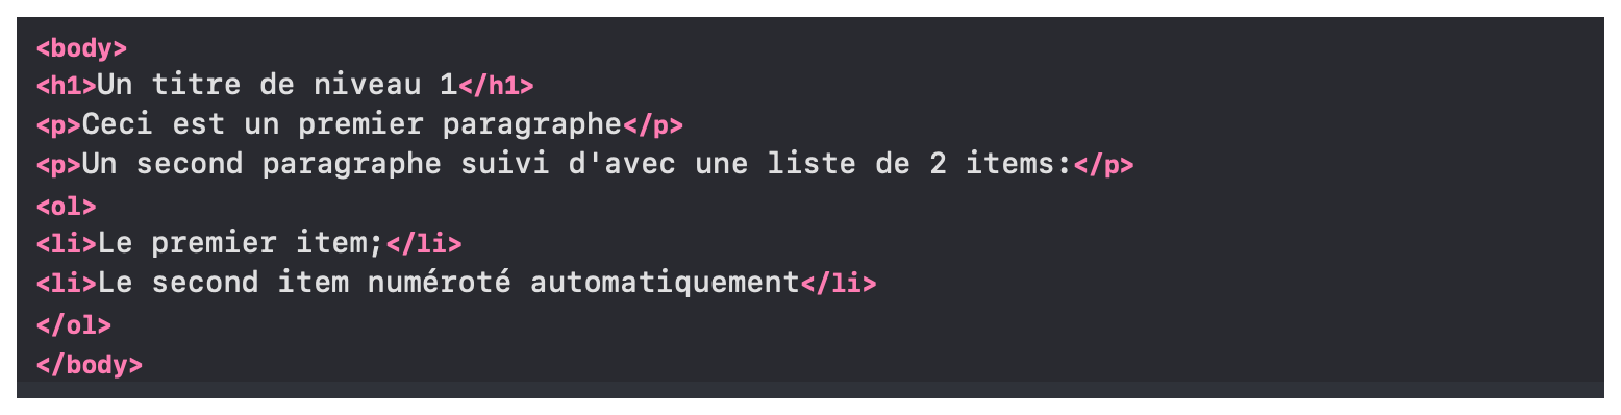
\includegraphics[scale=0.38]{img/exemple3-code.eps}
\end{center}
Qui affichera :
\begin{center}
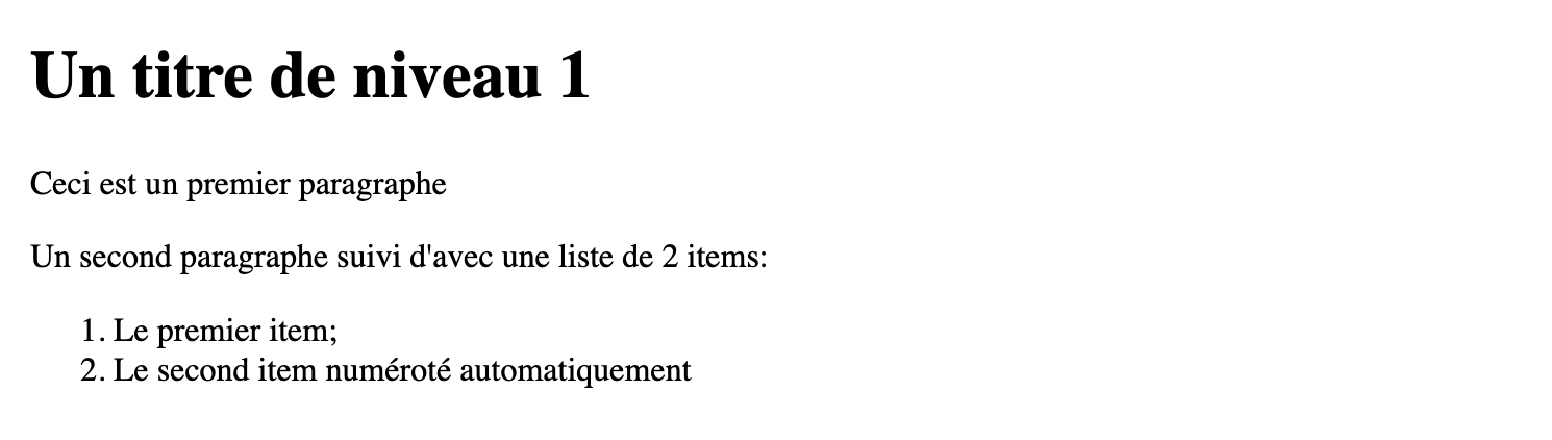
\includegraphics[scale=0.38]{img/exemple3.eps}
\end{center}
\end{exampleblock}
\end{frame}

\begin{frame}
\frametitle{Langage HTML}

\begin{block}{Balises de caractères}
\begin{itemize}
\item La mise en gras est balisée par \textbf{b} et la mise en italique est balisée par \textbf{i} 
\item La diminution de la police de caractère est balisée par \textbf{small}
\item La mise en indice d'un caractère est balisée par \textbf{sub} et la mise en exposant d'un caractère est balisée par  \textbf{sup}
\item La mise en forme d'un code de texte est balisée par \textbf{code}
\end{itemize}
\end{block}

\begin{block}{Balises de lien hypertexte et d'image}
\begin{itemize}
\item Un mot ou une phrase est transformé en lien hypertexte lorsqu'on l'entoure par la balise \textbf{a}. Il faut lui associer un attribut \textbf{href} qui contiendra l'adresse du document à relier.
\item Une image (photo) peut être intégrée à un document html en utilisant la balise vide \textbf{img}. Il faut lui associer un attribut \textbf{src} qui contiendra l'adresse de l'image à insérer.
\end{itemize}
\end{block}

\begin{alertblock}{Remarque}
Les balises html structurent et affichent les éléments demandés. L'apparence et la disposition des contenus devra être être géré par du CSS.
\end{alertblock}
\end{frame}

\begin{frame}
\frametitle{Langage HTML}

\begin{exampleblock}{Exemple}
Voici un code de document HTML complet :\medskip

\begin{minipage}{7.7cm}
\includegraphics[scale=0.37]{img/exemple4-code.eps}
\end{minipage}\hfill
\begin{minipage}{4.3cm}
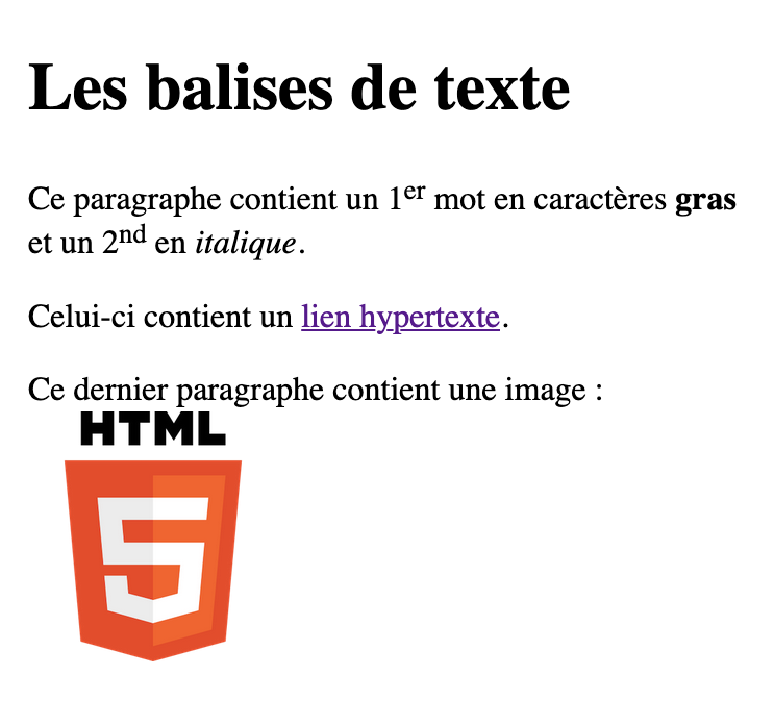
\includegraphics[scale=0.34]{img/exemple4.eps}
\end{minipage}

\end{exampleblock}

\end{frame}

\begin{frame}
\frametitle{Langage HTML}

\begin{block}{Balises de bloc}
\begin{enumerate}
\item On peut regrouper les contenus d'un document HTML dans des blocs. Ces blocs sont balisés par \textbf{div}.
\item Certain blocs ont une fonction bien précise et sont désignés par des balises spéciales.

On a par exemple :

\begin{itemize}
\item La balise \textbf{nav} qui est utilisée pour les menus.
\item La balise \textbf{aside} qui est utilisée pour la navigation à l'interieur d'un site WEB et souvent positionnée sur le coté de l'écran.
\item La balise \textbf{article} qui est utilisée pour le contenu entier d'un document avec un titre, plusieurs paragraphes, des liens et des images.
\item La balise \textbf{section} qui est utilisée pour organiser les contenus par section.
\item La balise \textbf{header} qui est utilisée pour créer un en-tête.
\item La balise \textbf{footer} qui est utilisée pour créer un pied de page.
\end{itemize}
\end{enumerate}

\end{block}

\begin{alertblock}{Remarques}
\begin{enumerate}
\item Ces balises de blocs peuvent s'imbriquer. Il est possible d'avoir plusieurs balises \textbf{articles} dans une balise \textbf{section}. On peut aussi avoir les balises \textbf{header} et \textbf{footer} dans une balise \textbf{article}.
\item Ces balises structurent le contenu et ne gèrent pas leur disposition.
\end{enumerate}

\end{alertblock}

\end{frame}


\begin{frame}
\frametitle{Langage HTML}

\begin{exampleblock}{Exemple}
\begin{minipage}{0.54\textwidth}
La structure donnée en exemple est imbriquée dans la balise $<\text{body}>$ du document html.

On peut réaliser la même structure en utilisant uniquement des blocs \textbf{div}. 

Pour les différencier il sera nécessaire de leur donner un identifiant ou \textbf{id}.

Par exemple, pour les deux articles, la structure sera :\medskip

\begin{center}
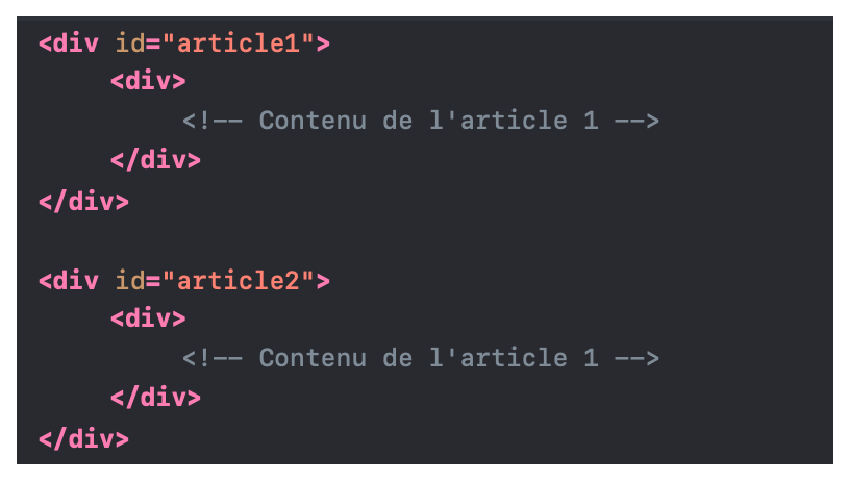
\includegraphics[scale=0.38]{img/exemple5-code.eps}
\end{center}

\textbf{Remarque:} L'image ci-contre représente la structure. La disposition des blocs sera obtenue uniquement avec du CSS.
\end{minipage}\hfill
\begin{minipage}{0.44\textwidth}
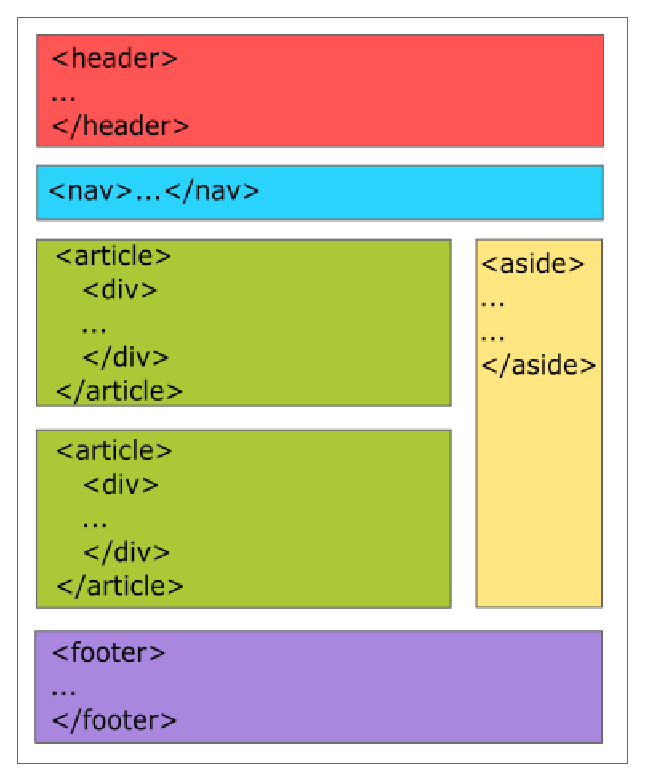
\includegraphics[scale=0.5]{img/structureHTML5.eps}
\end{minipage}

\end{exampleblock}

\end{frame}


%****************************************************************************
%
% Partie 2 : Langage CSS
%
%****************************************************************************

\begin{frame}
\frametitle{Langage CSS}

\begin{block}{Introduction}
Le langage CSS de l'anglais Cascading Style Sheets signifiant feuilles de style en cascade est un langage permettant de définir les propriétés graphiques des éléments HTML constituant une page Web. Cela permet par exemple :

\begin{itemize}
\item De modifier la police de caractère, sa taille, sa fonte, son alignement, sa couleur etc.
\item De modifier les couleurs des différents éléments HTML de la page comme les fonds.
\item De gérer les espacements entre les blocs et leurs dispositions.
\item D'ajouter des images de fond et des logos.
\end{itemize}
\end{block}

\begin{block}{La syntaxe CSS}
\begin{minipage}{0.7\textwidth}
L'application d'un style CSS se fait par le choix d'un \textbf{sélecteur} contenant, entre deux accolades, des couples \textbf{propriétés:valeurs} séparés par des points virgules.\medskip

Le nombre de propriétés n'est pas limité tant qu'elles existent.
\end{minipage}\hfill
\begin{minipage}{0.26\textwidth}
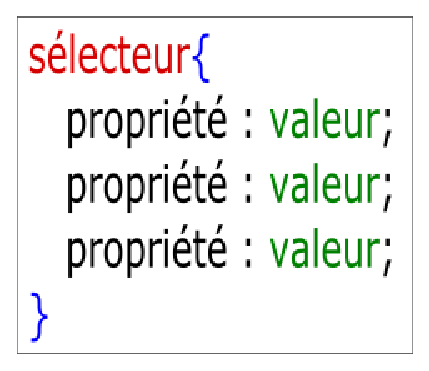
\includegraphics[scale=0.4]{img/selecteurCSS.eps}
\end{minipage}

\end{block}
\end{frame}

\begin{frame}
\frametitle{Langage CSS}

\begin{exampleblock}{Exemple}
\begin{minipage}{0.54\textwidth}
Voici le CORPS (body) d'un document en HTML:

\begin{center}
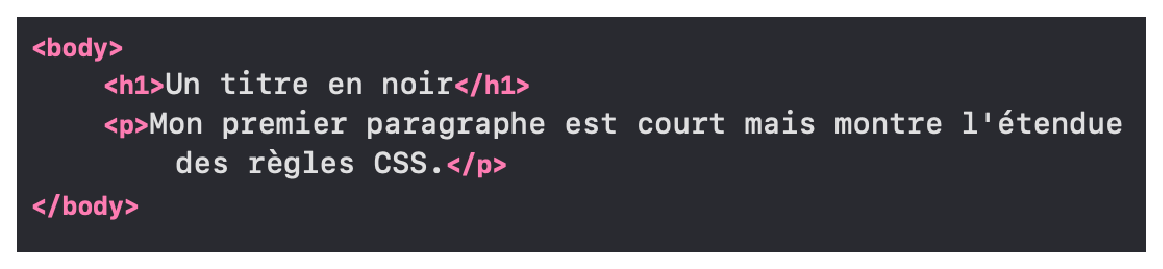
\includegraphics[scale=0.34]{img/exemple1-HTML.eps}
\end{center}

Voici des règles CSS associées aux sélecteurs \textbf{h1} et \textbf{p}:
\begin{center}
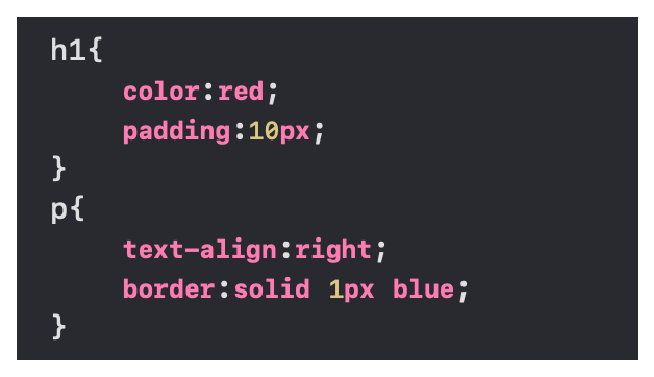
\includegraphics[scale=0.38]{img/exemple1-CSS.eps}
\end{center}
\end{minipage}\hfill
\begin{minipage}{0.42\textwidth}
Page HTML \textbf{avant} l'application des règles CSS:\medskip

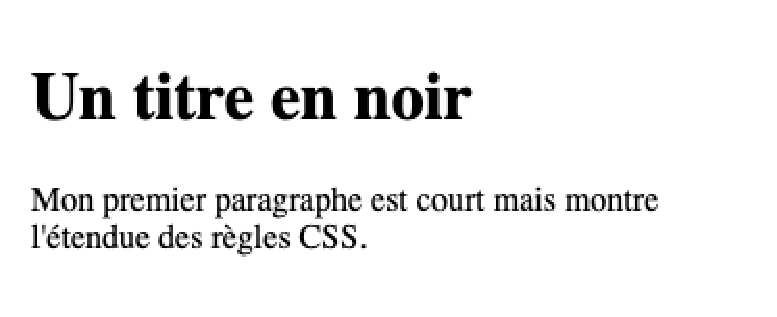
\includegraphics[scale=0.4]{img/exempleCSS1.eps}

Page HTML \textbf{après} l'application des règles CSS:\medskip

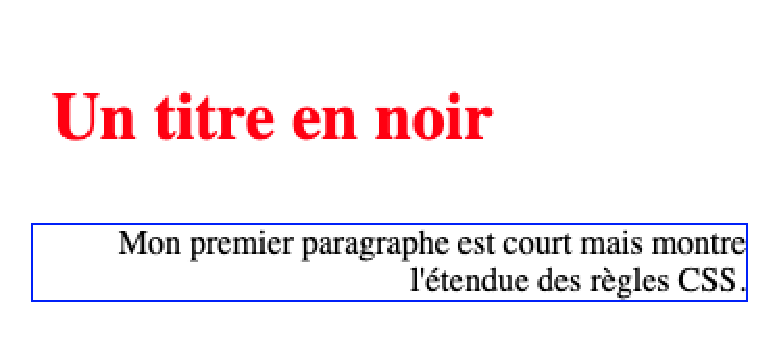
\includegraphics[scale=0.4]{img/exempleCSS2.eps}
\end{minipage}

\end{exampleblock}

\end{frame}


\begin{frame}
\frametitle{Langage CSS}

\begin{block}{Les sélecteurs CSS}
Il existe plusieurs manières de choisir un \textbf{sélecteur}.
\begin{enumerate}
\item En utilisant directement la balise html du document (comme l'exemple précédent).

Cette méthode est simple mais rencontre une difficulté. Les règles CSS seront appliquées à tous les sélecteurs de même type.

Dans l'exemple précédent, s'il y avait plusieurs paragraphes, ils seraient tous alignés à droite et encadrés en bleu !
\item En ajoutant un attribut \textbf{class} à l'élément HTML. Cette méthode offre 2 avantages:
\begin{itemize}
\item Tous les éléments qui ont la même classe ont les mêmes règles CSS appliquées.
\item Les éléments de même type peuvent avoir des règles CSS différentes en leur attribuant des classes différentes.
\end{itemize}
\item En donnant un \textbf{identifiant} aux éléments HTML du document. Chaque identifiant est unique donc les règles CSS ne s'appliqueront qu'à cet élément.
\item On peut attribuer des règles CSS en mélangeant les trois premières méthodes.

Un élément paragraphe $</\text{p}>$ peut avoir un identifiant et une class ce qui donne par exemple : $<\text{p id="premier" class="rouge"}>$
\end{enumerate}
\end{block}
\end{frame}

\begin{frame}
\frametitle{Langage CSS}

\begin{exampleblock}{Exemple}
\begin{minipage}{0.54\textwidth}
Voici un extrait de document en HTML:
\begin{center}
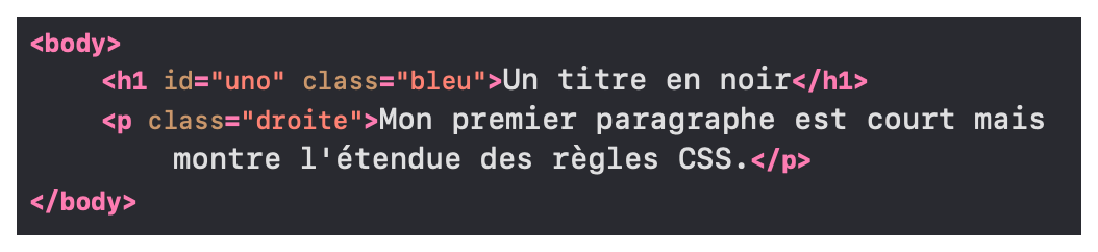
\includegraphics[scale=0.38]{img/exemple2-HTML.eps}
\end{center}

Voici des règles CSS associés aux sélecteurs :

\begin{center}
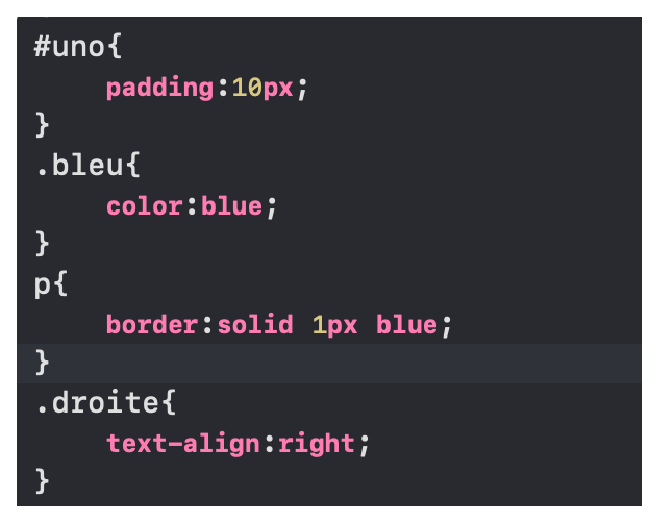
\includegraphics[scale=0.38]{img/exemple2-CSS.eps}
\end{center}
\end{minipage}\hfill
\begin{minipage}{0.42\textwidth}
Page HTML \textbf{avant} l'application des règles CSS:\medskip

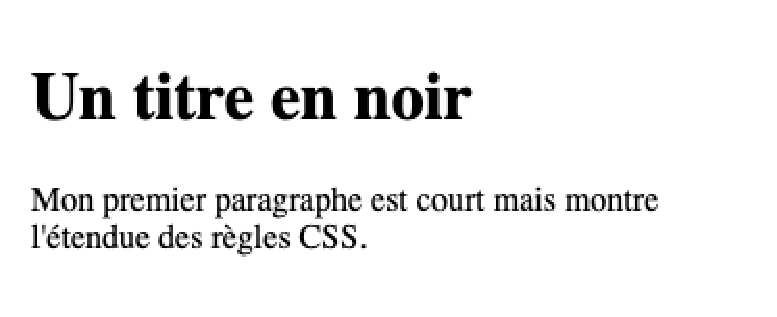
\includegraphics[scale=0.4]{img/exempleCSS1.eps}

Page HTML \textbf{après} l'application des règles CSS:\medskip

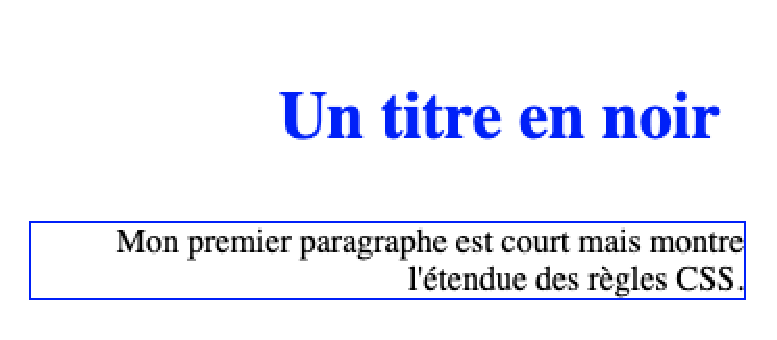
\includegraphics[scale=0.4]{img/exempleCSS3.eps}
\end{minipage}

\end{exampleblock}

\end{frame}

\begin{frame}
\frametitle{Langage CSS}

\begin{block}{Déclaration de style}
La première méthode se fait directement au niveau de la balise et les deux autres méthodes se font dans l'en-tête, entre les balises $<\text{head}>$ et $</\text{head}>$ du fichier html.
\medskip

\textbf{Méthode 1 :} dans la balise html, on insère l'attibut \textbf{style} et on lui donne en valeur les règles CSS.
\begin{center}
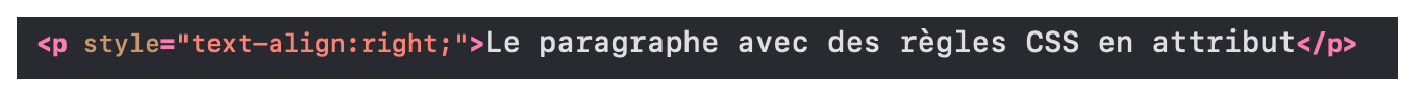
\includegraphics[scale=0.38]{img/exemple3-CSS.eps}
\end{center}


\textbf{Méthode 2 :} entre les balises $<\text{head}>$ et $</\text{head}>$ du fichier html, on ajoute les balises $<\text{style}>$ et $</\text{style}>$ contenant les propriétés CSS;
\begin{center}
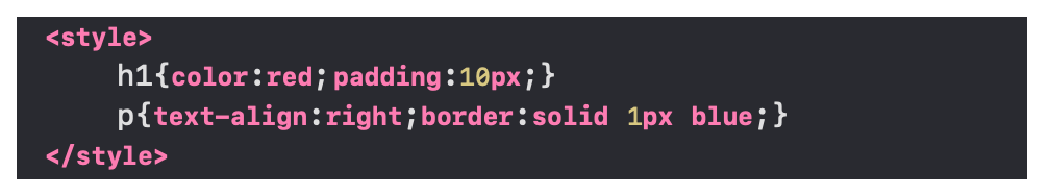
\includegraphics[scale=0.43]{img/exemple4-CSS.eps}
\end{center}

\textbf{Méthode 3 :} entre les balises $<\text{head}>$ et $</\text{head}>$ du fichier html, on ajoute la balise vide \textbf{link} et on crée un fichier \textbf{style.css} contenant toutes les règles CSS.
\begin{center}
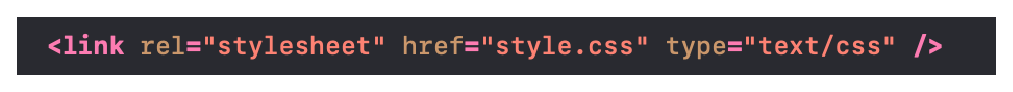
\includegraphics[scale=0.45]{img/exemple5-CSS.eps}
\end{center}

\end{block}
\end{frame}

\begin{frame}
\frametitle{Langage CSS}

\begin{block}{Positionnement des éléments HTML}
Les éléments HTML sont comme des boites avec du contenu. Les boites sont de 2 types :
\begin{itemize}
\item inline : les liens, le gras, les images, etc
\item block : les titres, les paragraphes, les div et les éléments nav, article, aside, etc.
\end{itemize}
Selon le type, l'affichage et le positionnement sont différents.
\begin{itemize}
\item Pour un élément HTML inline, il se comporte comme du texte.
\item Pour un élément HTML de type block, iloccupe toute la largeur de la page par défaut. Il faut attribuer des règles CSS pour avoir un positionnement particulier.
\end{itemize}
Des règles CSS permettent de gérer les espaces autour et dans les éléments HTML:

\begin{center}
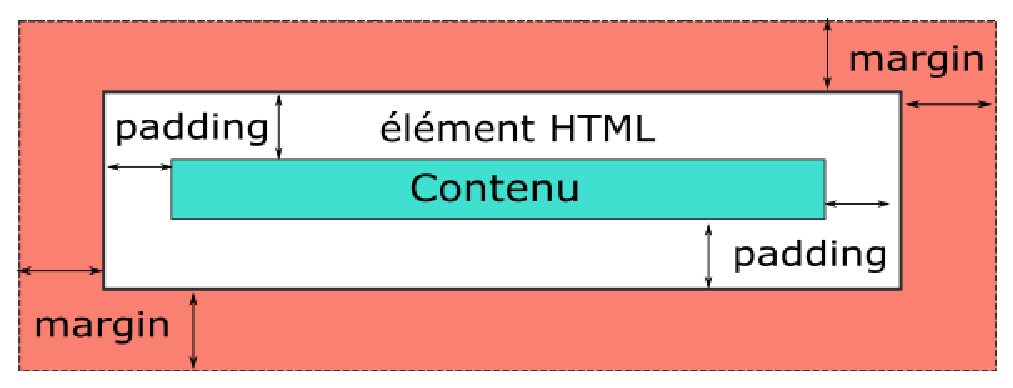
\includegraphics[scale=0.45]{img/margin-padding.eps}
\end{center}
\end{block}
\end{frame}





%****************************************************************************
%
% Partie 3 : Langage JAVASCRIPT
%
%****************************************************************************

\begin{frame}
\frametitle{Langage JAVASCRIPT}

\begin{block}{Présentation}
Le langage JAVASCRIPT a été créé par Brendan Eich en 1985 pour permettre aux navigateurs (FIREFOX, CHROME, ...) d'exécuter des programmes pour les documents WEB. 
\begin{itemize}
\item JAVASCRIPT est un un langage de programmation : des variables (numériques, chaines de caractères, tableaux,...), des conditions (if ... else), des boucles et des fonctions;
\item JAVASCRIPT permet de modifier le document HTML et les règles CSS du document;
\item JAVASCRIPT est à l'écoute d'événements qui sont liés aux actions du lecteur du document HTML : click de souris, déplacement de la souris, pression sur touche du clavier, chargement d'un document, ...
\item JAVASCRIPT peut faire des requêtes HTTP (formulaires).
\end{itemize}
\end{block}

\begin{block}{Déclaration}
Un script JAVASCRIPT se déclare avec la balise $<\text{script}>$ dans le HEAD du document HTML. Il existe deux méthodes :
\begin{itemize}
\item \textbf{Méthode 1:} le script JAVASCRIPT est inséré entre les balises $<\text{script}>$ et $</\text{script}>$.
\item \textbf{Méthode 2:} le script JAVASCRIPT est écrit dans un fichier externe d'extension JS et appelé par la balise $<\text{script src="js/monscript.js" type="text/javascript"}></\text{script}>$.
\end{itemize}
\end{block}
\end{frame}


\begin{frame}
\frametitle{Langage JAVASCRIPT}

\begin{block}{DOM}
Un document HTML est constitué de différents éléments html imbriqués les uns dans les autres. Cette structure peut se représenter par un arbre dont les noeuds sont les éléments html, (balises) reliés entre eux par des branches et les feuilles sont les contenus de texte. Cette structure s'appelle le DOM pour Document Object Model.
\end{block}

\begin{exampleblock}{Exemple}
Voici un code de document HTML et son DOM:\medskip

\begin{minipage}{7.7cm}
\includegraphics[scale=0.37]{img/exemple4-code.eps}
\end{minipage}\hfill
\begin{minipage}{4.3cm}
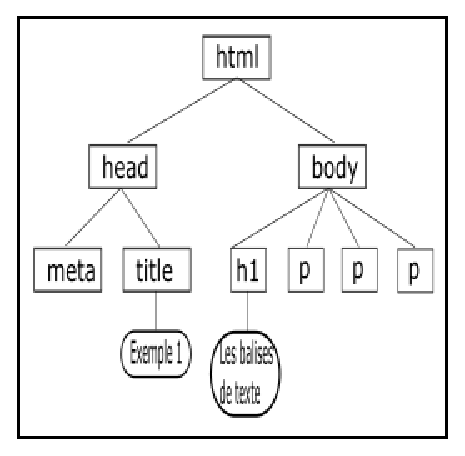
\includegraphics[scale=0.6]{img/dom.eps}
\end{minipage}

\end{exampleblock}
\end{frame}



\begin{frame}
\frametitle{Langage JAVASCRIPT}

\begin{block}{Parcourir le DOM}
Le script JAVASCRIPT ne peut s'éxécuter qu'à la fin du chargement de la page WEB. Ainsi, il est possible de parcourir le DOM du document pour y effectuer des modifications. La sélection des éléments se fait sur :
\begin{itemize}
\item Les sélecteurs : h1, p, a, div, etc.
\item Les identifiants des éléments html : id="identifiant"
\item Les class CSS appliquées aux sélecteurs : class="nom de classe"
\item Les éléments parents, enfants, frères, etc grace à des méthodes spécifiques.
\end{itemize} 
\end{block}

\begin{exampleblock}{Exemple}
Pour accéder à l'élément paragraphe \textbf{p}, on peut utiliser la méthode JAVASCRIPT
\textbf{querySelectorAll('sélecteur');}.\smallskip

Cete méthode va parcourir tout le DOM et sélectionner tous les éléments \textbf{p}. On obtient donc en résultat un tableau contenant chaque élément.\medskip

\hspace{0.5cm}\textbf{let} mesParagraphes = document.querySelectorAll('p');\\

\hspace{0.5cm}\textbf{for} (i=0 ; i < mesParagraphes.length ; i++) \{\\

\hspace{1cm}mesParagraphes[i].\textbf{style.color} = "blue";

\hspace{0.5cm}\}

\end{exampleblock}
\end{frame}



\end{document}
